\section*{Dati}

\noindent
\\Qui di seguito vengono riassunti in formato tabellare diversi \textit{parametri  termodinamici} relativi a ciascuno strato biologico trattato nel problema in esame.\\

\hspace{-1.5cm}
\begin{minipage}{\columnwidth}
\begin{table}[H]
\centering
\resizebox{1.1\columnwidth}{!}{%
\begin{tabular}{|ccc|c|}
\hline 
\phantom{     }              & \phantom{     } &  \phantom{}      &  \phantom{     }                       \\ 
\phantom{     }              & \Large{\textbf{PARAMETRI TERMODINAMICI}} &  \phantom{}      &  \Large{\textbf{STRATI BIOLOGICI } }                     \\ 
\phantom{     }              & \phantom{     } &  \phantom{}      &  \phantom{     }                       \\
\hline
\phantom{     }              & \phantom{     } &  \phantom{}      &  \phantom{     }                       \\ 
$T_{\infty} \;=\; 20\:$°C              & $h_{\infty}\: (T) \;=\; \bar{h_c} \;=\; 13.5\: W/(m^2K)$ & $u_{\infty} \;=\; 0.2 \: $m/s        & ARIA                       \\
\phantom{     }              & \phantom{     } &  \phantom{}      &  \phantom{     }                       \\ \hline
\phantom{     }              & \phantom{     } &  \phantom{}      &  \phantom{     }                       \\ 
$\rho_{ep} \;=\; 1000 \; kg/m^3 $ &
  $k_{ep} \;=\; 0.37 \; W/mK $ &
  $c_{ep} \;=\; 3391 \; J/kgK $ &
  \multirow{2}{*}{$\;$EPIDERMIDE - DERMA - SOTTOCUTE$\;$}    \\ 
$A \;=\; 1.80 \cdot 10^{50} \: s^{-1}$ & $\Delta H \;=\; 3.27 \cdot 10^5 \: J/mol$                & $\dot{Q}_{MET} \;=\; 400 \: W/m^3$   &    \phantom{   }                        \\ 
\phantom{     }              & \phantom{     } &  \phantom{}      &  \phantom{     }                       \\ \hline
\phantom{     }              & \phantom{     } &  \phantom{}      &  \phantom{     }                       \\ 
$\rho_{g} \;=\; 1041 \; kg/m^3 $ &
  $k_{g} \;=\; 0.33 \; W/mK $ &
  $c_{g} \;=\; 2960 \; J/kgK $ &
  \multirow{2}{*}{STRATO GHIANDOLARE}    \\ 
$A \;=\; 1.18 \cdot 10^{46} \: s^{-1}$ & $\Delta H \;=\; 3.02 \cdot 10^5 \: J/mol$                & $\dot{Q}_{MET} \;=\; 700 \: W/m^3$   &                            \\ 
\phantom{     }              & \phantom{     } &  \phantom{}      &  \phantom{     }                       \\ \hline
\phantom{     }              & \phantom{     } &  \phantom{}      &  \phantom{     }                       \\ 
$\rho_{t} \;=\; 1060 \; kg/m^3 $       & $k_{t} \;=\; 0.415 \; W/mK $                             & $c_{g} \;=\; 2726 \; J/kgK $        & \multirow{2}{*}{TUMORE}    \\ 
$A \;=\; 1.18 \cdot 10^{36} \: s^{-1}$ & $\Delta H \;=\; 2.38 \cdot 10^5 \: J/mol$                & $\dot{Q}_{MET} \;=\; 1400 \: W/m^3$  &                            \\ 
\phantom{     }              & \phantom{     } &  \phantom{}      &  \phantom{     }                       \\ \hline
\phantom{     }              & \phantom{     } &  \phantom{}      &  \phantom{     }                       \\ 
$\rho_{c} \;=\; 1102 \; kg/m^3 $       & $k_{c} \;=\; 0.46 \; W/mK $                              & $c_{c} \;=\; 3306 \; J/kgK $        & \multirow{2}{*}{CAPILLARE} \\ 
$A \;=\; 5.60 \cdot 10^{63} \: s^{-1}$ & $\Delta H \;=\; 4.30 \cdot 10^5 \: J/mol$                & $\dot{Q}_{MET} \;=\; 400 \: W/m^3$   &                            \\ 
\phantom{     }              & \phantom{     } &  \phantom{}      &  \phantom{     }                       \\ \hline
\phantom{     }              & \phantom{     } &  \phantom{}      &  \phantom{     }                       \\ 
$\rho_{b} \;=\; 1050 \; kg/m^3 $       & $-$                                                      & $c_{b} \;=\; 3617\; J/kgK $         & \multirow{2}{*}{SANGUE}    \\ 
$A \;=\; 5.60 \cdot 10^{63} \: s^{-1}$ & $\Delta H \;=\; 4.30 \cdot 10^5 \: J/mol$                & $u_{b} \;=\; 2 \cdot 10^{-4} \: $ m/s &                            \\ 
\phantom{     }              & \phantom{     } &  \phantom{}      &  \phantom{     }                       \\ \hline
\end{tabular}%
}
\end{table}
\end{minipage}

\noindent
\\\\\\Di seguito viene invece riportata una tabella che mostra i parametri che definiscono la \textit{geometria} del sistema.

\begin{adjustwidth}{0cm}{0cm}
	\begin{multicols}{2} % Divide la pagina in due colonne
		%\centering

        \hspace{-1.3cm}
        \begin{minipage}{\columnwidth}
        \begin{figure}[H]
        \centering
        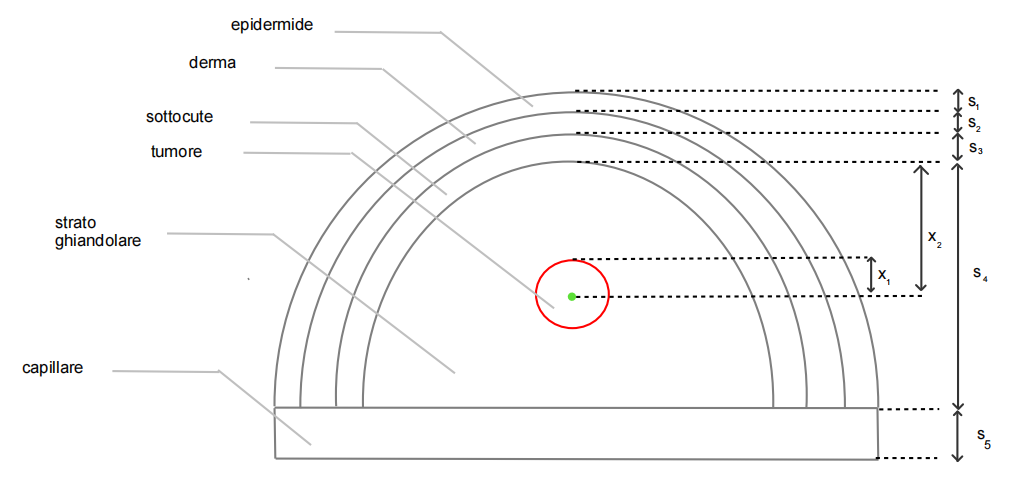
\includegraphics[scale = 0.5]{Immagini/geometria.png}
        \caption{Geometria}
        \label{geometria}
        \end{figure}
		\end{minipage}
  
		\columnbreak % Passa alla seconda colonna

        \hspace{1.5cm}
        \begin{minipage}{\columnwidth}
        \vspace{1.8cm}
        \begin{table}[H]
        \centering
        \resizebox{0.6\columnwidth}{!}{%
        \begin{tabular}{|c|}
        \hline
        \textbf{PARAMETRI GEOMETRICI} \\ \hline
        $s_1 \;=\; 3.5 \:mm$          \\ \hline
        $s_2 \;=\; 4.0 \:mm$          \\ \hline
        $s_3 \;=\; 3.5 \:mm$          \\ \hline
        $s_4 \;=\; 25 \:mm$           \\ \hline
        $s_5 \;=\; 10 \:\mu m$        \\ \hline
        $x_1 \;=\; 2 \:mm$            \\ \hline
        $x_2 \;=\; 10 \:mm$           \\ \hline
        \end{tabular}%
        }
        \end{table}
		\end{minipage}
  
	\end{multicols}
\end{adjustwidth}


\newpage